% 黎曼球面：球极投影与无穷远点
\documentclass[border=4pt]{standalone}
\usepackage{tikz}
\usetikzlibrary{arrows.meta}
\usepackage{amsmath,amssymb}
\definecolor{fillA}{rgb}{0.45,0.45,0.45}
\definecolor{fillB}{rgb}{0.72,0.72,0.72}
\begin{document}
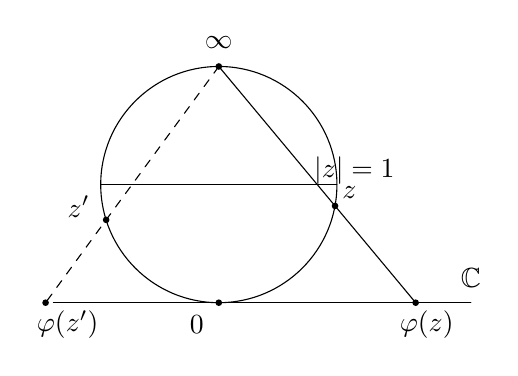
\begin{tikzpicture}[>=Stealth, line cap=round]
% 球面与复平面
\draw (2.7,2.6) circle (1.5);
\draw (0.6,1.1) -- (5.9,1.1);
\node at (5.9,1.42) {$\mathbb C$};
% 赤道 |z|=1
\draw (1.2,2.6) -- (4.2,2.6);
\node at (4.42,2.78) {$|z|=1$};
% 极点
\fill (2.7,4.1) circle (1.2pt);
\node at (2.7,4.4) {$\infty$};
\fill (2.7,1.1) circle (1.2pt);
\node at (2.42,0.82) {$0$};
% 球极投影：z
\fill (4.176,2.329) circle (1.2pt);
\node at (4.36,2.5) {$z$};
\draw (2.7,4.1) -- (4.176,2.329) -- (5.2,1.1);
\fill (5.2,1.1) circle (1.2pt);
\node at (5.34,0.82) {$\varphi(z)$};
% 球极投影：z'
\fill (1.269,2.152) circle (1.2pt);
\node at (0.92,2.32) {$z'$};
\draw[dashed] (2.7,4.1) -- (1.269,2.152) -- (0.5,1.1);
\fill (0.5,1.1) circle (1.2pt);
\node at (0.78,0.82) {$\varphi(z')$};
\end{tikzpicture}
\end{document}
